%-------------------------------------------------------------------------------
%                                PREAMBLE
%-------------------------------------------------------------------------------
\documentclass[usenames,dvipsnames,svgnames,10pt,aspectratio=169]{beamer}
%
\usefonttheme{professionalfonts}
% This theme uses TIKZ: compile twice with PDFLaTeX or LuaLaTeX.
%
%  Options:
%  - [clean]:    clean slides, i.e. logos and footbar are removed
%  - [kth]:      footbar style inspierd to the official KTH template
%  - [nicewave]: a different style of wave is used (not approved by FLOW)
%
\usetheme[clean]{flow}

\usepackage{tikz}
\usetikzlibrary{arrows}
\usetikzlibrary{shapes.geometric, math, positioning, calc, patterns, angles, quotes}
\usetikzlibrary{patterns.meta,decorations.pathmorphing}

\newcommand{\semaphore}[3]{% #1: color of circle,
                           % #2: color of semicircle
                           % #3: angle of semicircle 
  \tikz[node distance=0mm,baseline]
       {
         \node (s1) [circle, fill=#1, minimum size=6mm] {};
         \node      [semicircle, fill=#2, 
           inner sep=0pt, outer sep=0pt, minimum size=3mm,
           anchor=south,
           at={(s1.center)}, rotate=#3] {};
       }
}

\usepackage[]{circuitikz}

\usepackage{pgfplots}
\usepgfplotslibrary{polar}

\usepackage{hyperref,graphicx,lmodern}
\usepackage[utf8]{inputenc}
\usepackage{media9}
\usepackage{xcolor}
\usepackage{stmaryrd}
\usepackage{nicefrac}
\usepackage{multimedia}
\usepackage{multicol}
\usepackage{upgreek}
\usepackage[]{bm}
\usepackage[]{url}
\usepackage[]{animate}
\usepackage{amsmath}

\graphicspath{{imgs/}}
\setbeamertemplate{blocks}[rounded][shadow=true]

\DeclareMathOperator*{\maximize}{maximize~}

%-------------------------------------------------------------------------------
%                                TITLE PAGE
%-------------------------------------------------------------------------------
\title[Nonlinear physics] % Short title used in footline
{
	Poincaré-Lindstedt method \\
  for periodic dynamics
}

\author[J.-Ch.~Loiseau] % Presenting author in short form used in footline
{
	\underline{Jean-Christophe Loiseau}
}
% - Give the names in the same order as the appear in the paper.
% - Underline the presenting author.

\institute[unused]
{
	\url{jean-christophe.loiseau@ensam.eu} \\
	Laboratoire DynFluid \\
	Arts et M\'etiers, France.
}
% Keep it simple, no one is interested in your street address.

% University logo(s)
\logot{\includegraphics[width=.128\paperwidth]{DynFluid_logo}}  % Top logo
\logob{\includegraphics[width=0.128\paperwidth]{ENSAM_logo}} % Bottom logo
% \logoc[{\includegraphics[width=.128\paperwidth]{limsi}}]{\includegraphics[width=.128\paperwidth]{limsi}} % Corner logo
%
% Cover image: \cvrimg{x position}{y position}{cover image}
\cvrimg{.77}{.8}{\includegraphics[width=.4\paperwidth]{cover.png}}

\date[unused]{Physique non-lin\'eaire -- 2019-2020}

\begin{document}

\titleframe	% Print the title as the first slide

%-------------------------------------------------------------------------------
%                           PRESENTATION SLIDES
%-------------------------------------------------------------------------------

\begin{frame}[t, c]{Poincaré-Bendixson thereom}{Periodic orbit or not ?}
  \begin{minipage}{.68\textwidth}
    One of the fundamental theorem in dynamical system theory pertaining to the existence of periodic orbits in planar systems (i.e.\ two-dimensional systems).
  \end{minipage}%
  \hfill
  \begin{minipage}{.28\textwidth}
    \centering
    \includegraphics[width=\textwidth]{poincare}
  \end{minipage}

  \vspace{1cm}
\end{frame}

\begin{frame}[t, c]{How to study periodic dynamics ?}{The Poincaré-Lindstedt method}
  \begin{minipage}{.68\textwidth}
    Method developed by A.\ Lindstedt in the 1880's to approximate uniformly periodic solutions to ordinary differential equations in the context of celestial mechanics later refined by H.\ Poincaré.
  \end{minipage}%
  \hfill
  \begin{minipage}{.28\textwidth}
    \centering
    \includegraphics[width=\textwidth]{lindsted}
  \end{minipage}

  \vspace{1cm}
\end{frame}

\begin{frame}[t, c]{How to study periodic dynamics ?}{Example : the simple pendulum}
  \begin{minipage}{.68\textwidth}
    Starting from Newton's principles, the equations of motion are
    %
    \[
    \ddot{\theta} + \dfrac{g}{L} \sin(\theta) = 0.
    \]

    Introducing the rescaled time $\tau = \sqrt{\dfrac{g}{L}} t$, the governing equations are reduce to
    %
    \[
    \ddot{\theta} + \sin(\theta) = 0,
    \]
    %
    where the dot notation now denotes derivation w.r.t.\ $\tau$.
  \end{minipage}%
  \hfill
  \begin{minipage}{.28\textwidth}
    \centering
    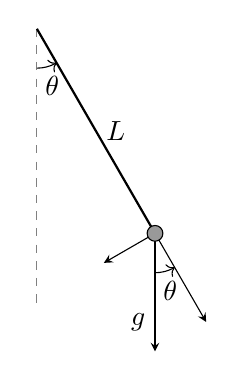
\begin{tikzpicture}
      % save length of g-vector and theta to macros
      \pgfmathsetmacro{\Gvec}{1.5}
      \pgfmathsetmacro{\myAngle}{30}
      % calculate lengths of vector components
      \pgfmathsetmacro{\Gcos}{\Gvec*cos(\myAngle)}
      \pgfmathsetmacro{\Gsin}{\Gvec*sin(\myAngle)}
      
      \coordinate (centro) at (0,0);
      \draw[dashed,gray,-] (centro) -- ++ (0,-3.5) node (mary) [black,below]{$ $};
      \draw[thick] (centro) -- ++(270+\myAngle:3) coordinate (bob) node[midway, right] {$L$};
      \pic [draw, ->, "$\theta$", angle eccentricity=1.5] {angle = mary--centro--bob};
      %\draw [blue,-stealth] (bob) -- ($(bob)!\Gcos cm!(centro)$);
      \draw [-stealth] (bob) -- ($(bob)!-\Gcos cm!(centro)$)
      coordinate (gcos)
      node[midway,above right] {};
      \draw [-stealth] (bob) -- ($(bob)!\Gsin cm!90:(centro)$)
      coordinate (gsin)
      node[midway,above left] {};
      \draw [-stealth] (bob) -- ++(0,-\Gvec)
      coordinate (g)
      node[near end,left] {$g$};
      \pic [draw, ->, "$\theta$", angle eccentricity=1.5] {angle = g--bob--gcos};
      \filldraw [fill=black!40,draw=black] (bob) circle[radius=0.1];
    \end{tikzpicture}
  \end{minipage}

  \vspace{1cm}
\end{frame}

\begin{frame}[t, c]{How to study periodic dynamics ?}{Example : the simple pendulum}
  \begin{minipage}{.68\textwidth}
    The exact period of oscillation for arbitrary initial angle can be expressed as
    %
    \[
    T = 4 \mathcal{F}\left( \dfrac{\pi}{2}, \sin \dfrac{\theta_0}{2} \right)
    \]
    %
    where $\mathcal{F}(\phi, k)$ is the incomplete elliptic integral of the first kind.

    \bigskip

    Although exact, this formula provides very limited insights into the dynamics\ldots
  \end{minipage}%
  \hfill
  \begin{minipage}{.28\textwidth}
    \centering
    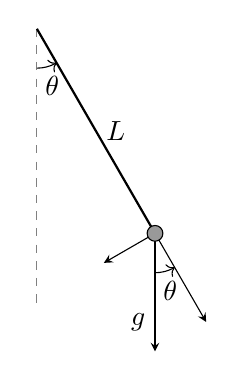
\begin{tikzpicture}
      % save length of g-vector and theta to macros
      \pgfmathsetmacro{\Gvec}{1.5}
      \pgfmathsetmacro{\myAngle}{30}
      % calculate lengths of vector components
      \pgfmathsetmacro{\Gcos}{\Gvec*cos(\myAngle)}
      \pgfmathsetmacro{\Gsin}{\Gvec*sin(\myAngle)}
      
      \coordinate (centro) at (0,0);
      \draw[dashed,gray,-] (centro) -- ++ (0,-3.5) node (mary) [black,below]{$ $};
      \draw[thick] (centro) -- ++(270+\myAngle:3) coordinate (bob) node[midway, right] {$L$};
      \pic [draw, ->, "$\theta$", angle eccentricity=1.5] {angle = mary--centro--bob};
      %\draw [blue,-stealth] (bob) -- ($(bob)!\Gcos cm!(centro)$);
      \draw [-stealth] (bob) -- ($(bob)!-\Gcos cm!(centro)$)
      coordinate (gcos)
      node[midway,above right] {};
      \draw [-stealth] (bob) -- ($(bob)!\Gsin cm!90:(centro)$)
      coordinate (gsin)
      node[midway,above left] {};
      \draw [-stealth] (bob) -- ++(0,-\Gvec)
      coordinate (g)
      node[near end,left] {$g$};
      \pic [draw, ->, "$\theta$", angle eccentricity=1.5] {angle = g--bob--gcos};
      \filldraw [fill=black!40,draw=black] (bob) circle[radius=0.1];
    \end{tikzpicture}
  \end{minipage}

  \vspace{1cm}
\end{frame}


\begin{frame}[t, c]{How to study periodic dynamics ?}{Example : the simple pendulum}
  \begin{minipage}{.48\textwidth}
    For infinitesimally small angles $\theta$, $\sin(\theta) \simeq \theta$.
    The system reduces to the \alert{\textbf{harmonic oscillator}}
    %
    \[
    \ddot{\theta} + \theta = 0
    \]
    %
    Its solution reads $\theta(t) = \theta_0 \cos(t)$ (assuming $\dot{\theta}(0) = 0$).
  \end{minipage}%
  \hfill
  \begin{minipage}{.48\textwidth}
    \centering
    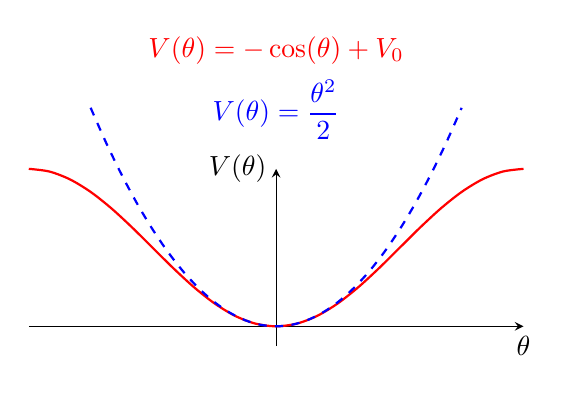
\begin{tikzpicture}[>=stealth]
      \draw[->] (-pi, 0) -- (pi, 0) node[below] {$\theta$};
      \draw[->] (0, -0.25) -- (0, 2) node[left] {$V(\theta)$};

      \draw[red, domain=-pi:pi, variable=\x, thick, smooth] plot (\x, {-cos(\x r) + 1}) {};
      \draw[blue, dashed, domain=-3*pi/4:3*pi/4, variable=\x, thick, smooth] plot (\x, {0.5 * \x * \x});

      \node[red] at (0, 3.5) {$V(\theta) = - \cos(\theta) + V_0$};
      \node[blue] at (0, 2.75) {$V(\theta) = \dfrac{\theta^2}{2}$};
    \end{tikzpicture}
  \end{minipage}

  \vspace{1cm}
\end{frame}


\begin{frame}[t, c]{How to study periodic dynamics ?}{Example : the simple pendulum}
  \begin{minipage}{.48\textwidth}
    Tthe second-order Taylor expansion of $\sin(\theta)$ yields
    %
    \[
    \ddot{\theta} + \theta - \dfrac{1}{6} \theta^3 = 0.
    \]

    It is known as \alert{\textbf{Duffing oscillator}}.
    Its exact solution can be expressed in terms of \alert{\textbf{elliptic Jacobi functions}}.
  \end{minipage}%
  \hfill
  \begin{minipage}{.48\textwidth}
    \centering
    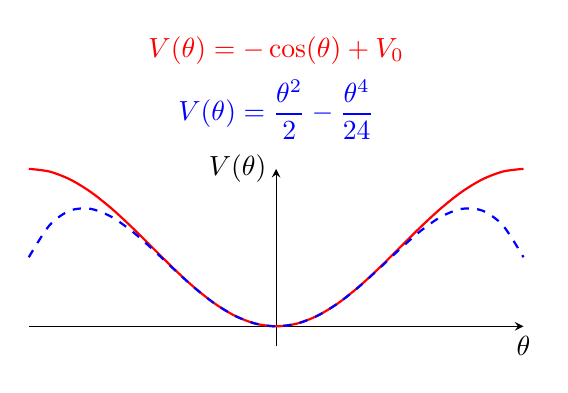
\begin{tikzpicture}[>=stealth]
      \draw[->] (-pi, 0) -- (pi, 0) node[below] {$\theta$};
      \draw[->] (0, -0.25) -- (0, 2) node[left] {$V(\theta)$};

      \draw[red, domain=-pi:pi, variable=\x, thick, smooth] plot (\x, {-cos(\x r) + 1}) {};
      \draw[blue, dashed, domain=-pi:pi, variable=\x, thick, smooth] plot (\x, {0.5 * \x * \x - (1/24)*(\x)^4});

      \node[red] at (0, 3.5) {$V(\theta) = - \cos(\theta) + V_0$};
      \node[blue] at (0, 2.75) {$V(\theta) = \dfrac{\theta^2}{2} - \dfrac{\theta^4}{24}$};
    \end{tikzpicture}
  \end{minipage}

  \vspace{1cm}
\end{frame}


\begin{frame}[t, c]{How to study periodic dynamics ?}{Example : the simple pendulum}
  \begin{minipage}{.68\textwidth}
    Introducing the change of variable $\theta(t) = \theta_0 x(t)$, the equation of motion can be written as
    %
    \[
    \left\{
    \begin{aligned}
      \ddot{x} + x & = \epsilon x^3 \\
      x(0) & = 1 \\
      \dot{x}(0) & = 0
    \end{aligned}
    \right.
    \]
    %
    where $\epsilon = \dfrac{\theta_0^2}{6}$.
    For $\epsilon$ sufficiently small, the nonlinear term can be understood as a small perturbation of the harmonic oscillator.
  \end{minipage}%
  \hfill
  \begin{minipage}{.28\textwidth}
    \centering
    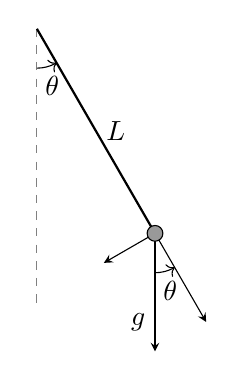
\begin{tikzpicture}
      % save length of g-vector and theta to macros
      \pgfmathsetmacro{\Gvec}{1.5}
      \pgfmathsetmacro{\myAngle}{30}
      % calculate lengths of vector components
      \pgfmathsetmacro{\Gcos}{\Gvec*cos(\myAngle)}
      \pgfmathsetmacro{\Gsin}{\Gvec*sin(\myAngle)}
      
      \coordinate (centro) at (0,0);
      \draw[dashed,gray,-] (centro) -- ++ (0,-3.5) node (mary) [black,below]{$ $};
      \draw[thick] (centro) -- ++(270+\myAngle:3) coordinate (bob) node[midway, right] {$L$};
      \pic [draw, ->, "$\theta$", angle eccentricity=1.5] {angle = mary--centro--bob};
      %\draw [blue,-stealth] (bob) -- ($(bob)!\Gcos cm!(centro)$);
      \draw [-stealth] (bob) -- ($(bob)!-\Gcos cm!(centro)$)
      coordinate (gcos)
      node[midway,above right] {};
      \draw [-stealth] (bob) -- ($(bob)!\Gsin cm!90:(centro)$)
      coordinate (gsin)
      node[midway,above left] {};
      \draw [-stealth] (bob) -- ++(0,-\Gvec)
      coordinate (g)
      node[near end,left] {$g$};
      \pic [draw, ->, "$\theta$", angle eccentricity=1.5] {angle = g--bob--gcos};
      \filldraw [fill=black!40,draw=black] (bob) circle[radius=0.1];
    \end{tikzpicture}
  \end{minipage}

  \vspace{1cm}
\end{frame}

\begin{frame}[t, c]{The Poincaré-Lindstedt method}{Example : the simple pendulum}
  Let us rescale time as $\tau = \omega t$ such that
  %
  \[
  \dfrac{d}{dt} = \omega \dfrac{d}{d\tau}, \quad \text{and} \quad \dfrac{d^2}{dt^2} = \omega^2 \dfrac{d^2}{d\tau^2}.
  \]
  %
  and use a power series expansion of the unknown frequency $\omega$ and solution $x(t)$
  %
  \[
  \begin{aligned}
    \omega & = 1 + \epsilon \omega_1 + \epsilon^2 \omega_2 + \cdots \\
    x(\tau) & = x_0(\tau) + \epsilon x_1(\tau) + \epsilon^2 x_2(\tau) + \cdots
  \end{aligned}
  \]
  %
  where $x_1(\tau)$ and $x_2(\tau)$ are small corrections to the harmonic oscillator solution $x_0(\tau)$ and $\omega_1$ and $\omega_2$ are small corrections to its natural frequency.

  \vspace{1cm}
\end{frame}

\begin{frame}[t, c]{The Poincaré-Lindstedt method}{Example : the simple pendulum}
  \begin{minipage}{.68\textwidth}
    Introducing these expansions into our equation and regrouping by power of $\epsilon$ yields
    %
    \[
    \begin{aligned}
      \mathcal{O}(\epsilon^0) : \quad \ddot{x}_0 + x_0 & = 0, \\
      \mathcal{O}(\epsilon^1) : \quad \ddot{x}_1 + x_1 & = x_0^3 - 2\omega_1 \ddot{x}_0, \\
      \mathcal{O}(\epsilon^2) : \quad \ddot{x}_2 + x_2 & = 3x_0^2 x_1 - 2\omega \ddot{x}_1 - (2\omega_2 + \omega_1^2) \ddot{x}_0 \\
    \end{aligned}
    \]
    %
    supplemented with the initial conditions
    %
    \[
    x_0(0) = 1, \quad \dot{x}_0(0) = 0, \quad x_i(0) = \dot{x}_i(0) = 0 \quad \forall i > 0.
    \]

    We have thus traded a nonlinear system for a cascade of linear systems we can solve sequentially !
  \end{minipage}%
  \hfill
  \begin{minipage}{.28\textwidth}
    \centering
    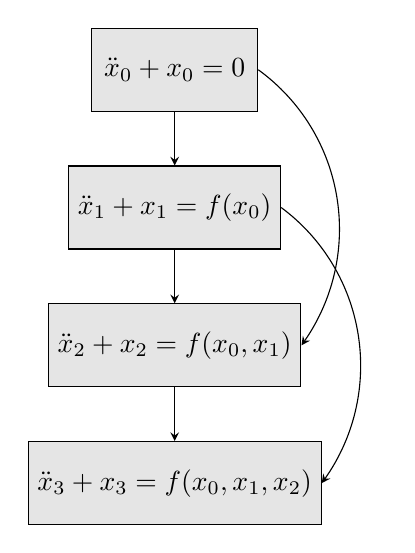
\begin{tikzpicture}[>=stealth]
      \tikzstyle{block} = [draw, fill=gray!20, rectangle, 
        minimum height=3em, minimum width=6em]

      \node [block, name=zeroth] {$\ddot{x}_0 + x_0 = 0$};
      \node [block, name=first, below of=zeroth, node distance=1.75cm] {$\ddot{x}_1 + x_1 = f(x_0)$};
      \node [block, name=second, below of=first, node distance=1.75cm] {$\ddot{x}_2 + x_2 = f(x_0, x_1)$};
      \node [block, name=third, below of=second, node distance=1.75cm] {$\ddot{x}_3 + x_3 = f(x_0, x_1, x_2)$};

      \draw[->] (zeroth) -- (first);
      \draw[->] (first) -- (second);
      \draw[->] (second) -- (third);
      \draw[->, bend right] (zeroth.east) to [out=45, in=135] (second.east);
      \draw[->, bend right] (first.east) to [out=45, in=135] (third.east);
    \end{tikzpicture}
  \end{minipage}

  \vspace{1cm}
\end{frame}

\begin{frame}[t, c]{The Poincaré-Lindstedt method}{Example : the simple pendulum}
  \begin{minipage}{.58\textwidth}
    The zeroth-order solution is simply given by $x_0(\tau) = \cos(\tau)$.
    Injecting $x_0(\tau)$ into the equation for $x_1(\tau)$ yields
    %
    \[
    \ddot{x}_1 + x_1 = \cos^3(\tau) + 2\omega_1 \cos(\tau)
    \]
    %
    which can be simplified to
    %
    \[
    \ddot{x}_1 + x_1 = \left( \dfrac{3}{4} + 2\omega_1 \right) \cos(\tau) + \dfrac{1}{4} \cos(3\tau)
    \]
    %
    using trigonometric identities.
  \end{minipage}%
  \hfill
  \begin{minipage}{.38\textwidth}
    \centering
    \textbf{Trig.\ identity}
    %
    \[
    \cos^3(\tau) = \dfrac{1}{4}\left( 3 \cos(\tau) + \cos(3\tau) \right)
    \]
  \end{minipage}

  \vspace{1cm}
\end{frame}

\begin{frame}[t, c]{The Poincaré-Lindstedt method}{Example : the simple pendulum}
  \begin{minipage}{.68\textwidth}
    If left unchecked, the $\cos(\tau)$ forcing term will lead to \alert{\textbf{secular growth}} (i.e. $x_1(\tau) \to \infty$ as $\tau \to \infty$) which is unphysical.
    We can however set the first-order frequency correction to
    %
    \[
    \omega_1 = - \dfrac{3}{8}
    \]
    %
    to avoid this unphysical behaviour (see the \alert{\textbf{Fredholm theorem}} for a theoretical justification).
  \end{minipage}%
  \hfill
  \begin{minipage}{.28\textwidth}
    \centering
    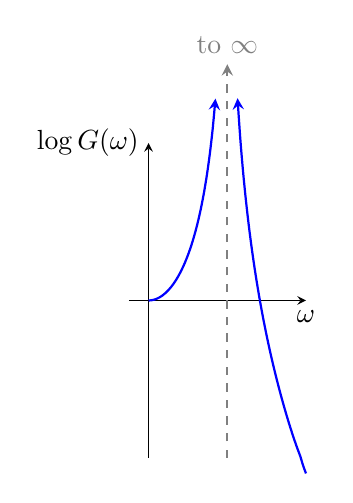
\begin{tikzpicture}[>=stealth]
      \draw[->] (-0.25, 0) -- (2, 0) node[below] {$\omega$};
      \draw[->] (0, -2) -- (0, 2) node[left] {$\log G(\omega)$};

      \draw[->, blue, thick, smooth, domain=0:0.85, variable=\x] plot (\x, {ln(1/(1-\x*\x)^2)});
      \draw[<-, blue, thick, smooth, domain=1.13:2, variable=\x] plot (\x, {ln(1/(1-\x*\x)^2)});

      \draw[->, dashed, gray, smooth, thick] (1, -2) -- (1, 3) node[above] {to $\infty$};

    \end{tikzpicture}
  \end{minipage}

  \vspace{1cm}
\end{frame}

\begin{frame}[t, c]{The Poincaré-Lindstedt method}{Example : the simple pendulum}
  \begin{minipage}{.68\textwidth}
    At order $\mathcal{O}(\epsilon)$, the equation then reduces to
    %
    \[
    \ddot{x}_1 + x_1 = \frac{1}{4} \cos(3\tau)
    \]
    %
    whose solution is given by $x_1(\tau) = \dfrac{1}{32} \left( \cos(\tau) - \cos(3\tau) \right)$.
    The first-order approximation to the true solution is thus given by
    %
    \[
    x(\tau) = \cos(\tau) + \dfrac{\epsilon}{32} \left( \cos(\tau) - \cos(3\tau)  \right) + \mathcal{O}(\epsilon^2)
    \]
    %
    with $\tau = \left( 1 - \dfrac{3\epsilon}{8} + \cdots \right) t$ our rescaled time.
  \end{minipage}%
  \hfill
  \begin{minipage}{.28\textwidth}
    \centering
    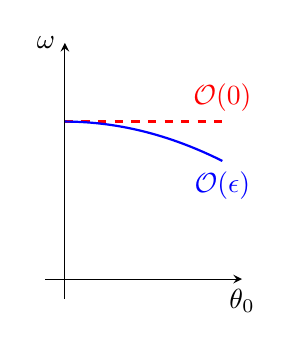
\begin{tikzpicture}[>=stealth]
      \draw[->] (-0.25, 0) -- (2.25, 0) node[below] {$\theta_0$};
      \draw[->] (0, -0.25) -- (0, 3) node[left] {$\omega$};

      \draw[red, thick, dashed] (0, 2) -- (2, 2) node[above] {$\mathcal{O}(0)$};
      \draw[blue, thick, smooth, domain=0:2, variable=\x] plot (\x, {2*(1 - 3*\x*\x / (8*6))}) node[below] {$\mathcal{O}(\epsilon)$};

    \end{tikzpicture}
  \end{minipage}

  \vspace{1cm}
\end{frame}

\begin{frame}[t, c]{The Poincaré-Lindstedt method}{Example : the simple pendulum}
  \begin{minipage}{.68\textwidth}
    Continuing this process for $\mathcal{O}(\epsilon^2)$ would yield the second-order frequency correction and an expression for $x(t)$ involving $\cos(\omega t)$, $\cos(3\omega t)$ and $\cos(5\omega t)$.

    \bigskip

    As $\epsilon$ is increased, the evolution of $x(t)$ is no longer a pure sine wave.
    The nonlinearity causes a \alert{\textbf{frequency shift}} as well as the generation of \alert{\textbf{higher-order harmonics}} !
  \end{minipage}%
  \hfill
  \begin{minipage}{.28\textwidth}
    \centering
    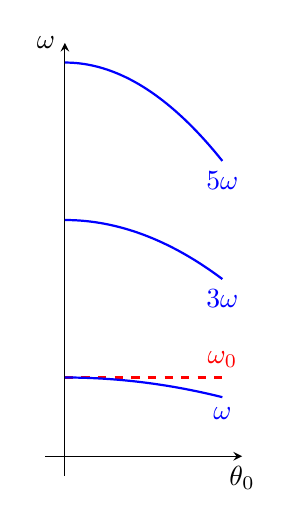
\begin{tikzpicture}[>=stealth]
      \draw[->] (-0.25, 0) -- (2.25, 0) node[below] {$\theta_0$};
      \draw[->] (0, -0.25) -- (0, 5.25) node[left] {$\omega$};

      \draw[red, thick, dashed] (0, 1) -- (2, 1) node[above] {$\omega_0$};
      \draw[blue, thick, smooth, domain=0:2, variable=\x] plot (\x, {(1 - 3*\x*\x / (8*6))}) node[below] {$\omega$};
      \draw[blue, thick, smooth, domain=0:2, variable=\x] plot (\x, {3*(1 - 3*\x*\x / (8*6))}) node[below] {$3\omega$};
      \draw[blue, thick, smooth, domain=0:2, variable=\x] plot (\x, {5*(1 - 3*\x*\x / (8*6))}) node[below] {$5\omega$};

    \end{tikzpicture}
  \end{minipage}

  \vspace{1cm}
\end{frame}

\begin{frame}[t, c]{The Poincaré-Lindstedt method}{Example : the simple pendulum}
  \begin{overprint}
    \onslide<1>
    \centering
    \begin{tikzpicture}[>=stealth]
      \draw[->] (-1.25*pi, 0) -- (1.25*pi, 0) node[below] {$\theta$};
      \draw[->] (0, -pi) -- (0, pi) node[left] {$\dot{\theta}$};
      
      \draw[gray, smooth, thick] plot file{pendulum_traj_1.txt};
      \draw[gray, smooth, thick] plot file{pendulum_traj_2.txt};
      \draw[gray, smooth, thick] plot file{pendulum_traj_3.txt};
      \draw[gray, smooth, thick] plot file{pendulum_traj_4.txt};
      \draw[gray, smooth, thick] plot file{pendulum_traj_5.txt};
      
      \draw[blue, dashed, smooth, thick] plot file{harmonic_traj_1.txt};
      \draw[blue, dashed, smooth, thick] plot file{harmonic_traj_2.txt};
      \draw[blue, dashed, smooth, thick] plot file{harmonic_traj_3.txt};
      \draw[blue, dashed, smooth, thick] plot file{harmonic_traj_4.txt};
      
      \node[circle, fill=black, draw=black, inner sep=0pt, minimum size=4pt] at (0, 0) {};
      \node[circle, fill=white, draw=black, inner sep=0pt, minimum size=4pt] at (-pi, 0) {};
      \node[circle, fill=white, draw=black, inner sep=0pt, minimum size=4pt] at (pi, 0) {};
      
      \draw[gray, thick] (pi/4, pi-0.5) -- (pi/4+1, pi-0.5) node[right] {True solution};
      \draw[dashed, blue, thick] (-pi/4, pi-0.5) -- (-pi/4-1, pi-0.5) node[left] {Harm.\ osc.};
    \end{tikzpicture}


    \onslide<2>
    \centering
    \begin{tikzpicture}[>=stealth]
      \draw[->] (-1.25*pi, 0) -- (1.25*pi, 0) node[below] {$\theta$};
      \draw[->] (0, -pi) -- (0, pi) node[left] {$\dot{\theta}$};
      
      \draw[gray, smooth, thick] plot file{pendulum_traj_1.txt};
      \draw[gray, smooth, thick] plot file{pendulum_traj_2.txt};
      \draw[gray, smooth, thick] plot file{pendulum_traj_3.txt};
      \draw[gray, smooth, thick] plot file{pendulum_traj_4.txt};
      \draw[gray, smooth, thick] plot file{pendulum_traj_5.txt};
      
      \draw[blue, dashed, smooth, thick] plot file{approx_traj_1.txt};
      \draw[blue, dashed, smooth, thick] plot file{approx_traj_2.txt};
      \draw[blue, dashed, smooth, thick] plot file{approx_traj_3.txt};
      \draw[blue, dashed, smooth, thick] plot file{approx_traj_4.txt};
      
      \node[circle, fill=black, draw=black, inner sep=0pt, minimum size=4pt] at (0, 0) {};
      \node[circle, fill=white, draw=black, inner sep=0pt, minimum size=4pt] at (-pi, 0) {};
      \node[circle, fill=white, draw=black, inner sep=0pt, minimum size=4pt] at (pi, 0) {};
      
      \draw[gray, thick] (pi/4, pi-0.5) -- (pi/4+1, pi-0.5) node[right] {True solution};
      \draw[dashed, blue, thick] (-pi/4, pi-0.5) -- (-pi/4-1, pi-0.5) node[left] {$\mathcal{O}(\epsilon)$};
    \end{tikzpicture}
  \end{overprint}
  \vspace{1cm}
\end{frame}


\begin{frame}[t, c]{The Poincaré-Lindstedt method}{Summary}
  \begin{minipage}{.68\textwidth}
    The Poincaré-Lindstedt method is a powerful perturbative technique to approximate periodic solutions to ordinary differential equations.

    \bigskip

    By rescaling time as $\tau = \omega t$ and using power series expansions, it transforms a nonlinear system into a cascade of linear ones which we can easily solve.

    \bigskip

    The resulting approximation provides insights into the frequency shift phenomenon and harmonics generation induced by the nonlinearity.
  \end{minipage}%
  \hfill
  \begin{minipage}{.28\textwidth}
    \centering
    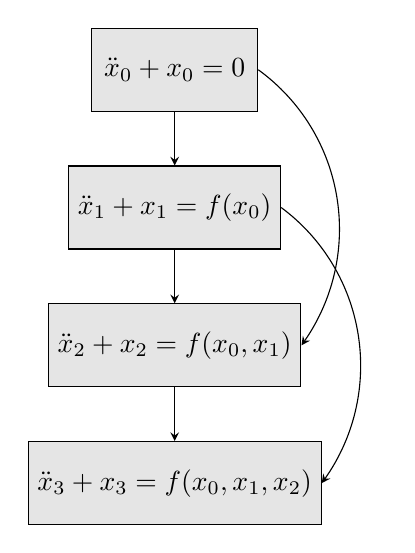
\begin{tikzpicture}[>=stealth]
      \tikzstyle{block} = [draw, fill=gray!20, rectangle, 
        minimum height=3em, minimum width=6em]

      \node [block, name=zeroth] {$\ddot{x}_0 + x_0 = 0$};
      \node [block, name=first, below of=zeroth, node distance=1.75cm] {$\ddot{x}_1 + x_1 = f(x_0)$};
      \node [block, name=second, below of=first, node distance=1.75cm] {$\ddot{x}_2 + x_2 = f(x_0, x_1)$};
      \node [block, name=third, below of=second, node distance=1.75cm] {$\ddot{x}_3 + x_3 = f(x_0, x_1, x_2)$};

      \draw[->] (zeroth) -- (first);
      \draw[->] (first) -- (second);
      \draw[->] (second) -- (third);
      \draw[->, bend right] (zeroth.east) to [out=45, in=135] (second.east);
      \draw[->, bend right] (first.east) to [out=45, in=135] (third.east);
    \end{tikzpicture}
  \end{minipage}

  \vspace{1cm}
\end{frame}

\end{document}
